\hypertarget{software-design-and-architecture-document-sda}{%
\section{Software Design and Architecture Document
(SDA)}\label{software-design-and-architecture-document-sda}}

\textbf{Authors:} Jake Goodwin, Aidan Agee, Blake Babb, Patrick Iacob

\textbf{DATE:} 2023-12-03

\hypertarget{introduction}{%
\subsection{Introduction}\label{introduction}}

This document establishes the software and hardware architecture for a
personal data acquisition system. Selecting the correct architecture
improves development velocity and enables more robust functionality by
having systems that support each other. Cohesive Software Architecture
is particularly important for this project as our workflow has
contributors split into two sub teams which are developing a frontend
and backend that must communicate. In addition to that, designing an
appropriate hardware architecture will reduce development costs and help
our product find its place in the market.

\hypertarget{architectural-goals-and-principles}{%
\subsection{Architectural Goals and
Principles}\label{architectural-goals-and-principles}}

Our hardware and software architectures have the primary goal of being
synergistic with each other and possessing libraries that interface with
each other.

Because our project covers layers ranging from hardware to a website,
connection throughout the stack is critical. Additionally, as we work
through the prototyping stage our architecture will practice modularity
to be able to add new sensor hardware as we expand the capabilities of
the product. Our architecture does not need to prioritize scalability as
the final objective is only to develop a prototype.

\hypertarget{system-overview}{%
\subsection{System Overview}\label{system-overview}}

\begin{figure}
\centering
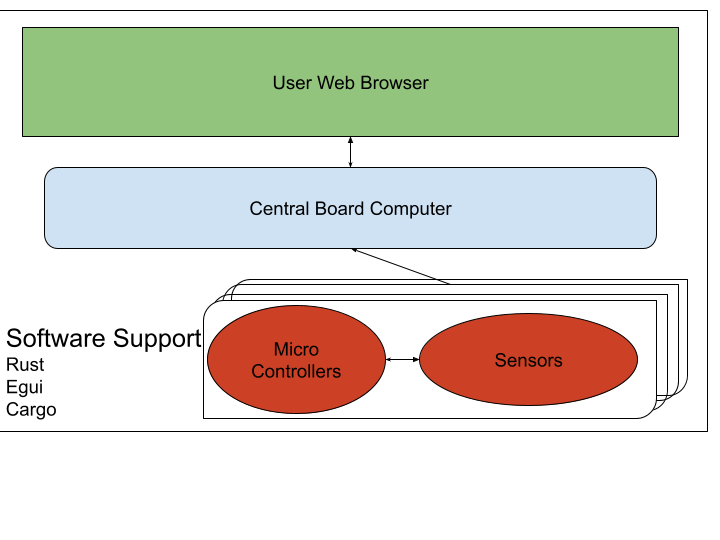
\includegraphics{SystemOverview.png}
\caption{image}
\end{figure}

\hypertarget{architectural-patterns}{%
\subsection{Architectural Patterns}\label{architectural-patterns}}

Controller Responder: This pattern is useful as our hardware SBC can act
as the controller which has a single responder in the user webpage. This
pattern would help cache data generated by the controller to provide a
seamless experience to the user in the face of latency issues.
Additionally, the ability to access data in the responder without
affecting the controller will allow for computation in an environment
separate from the hardware board.

Event Sourcing: This pattern works especially well with real-time data,
which is what this project is all about. Our hardware controller can act
as the producer and broadcast its data to a web server which will act as
the event source for an y users that want to query the server and
consume that data. The fail-safety of this design is also important to
this project as data acquisition environments, such as racing or
aeronautics, often cause damage to the controller while still requiring
data to be accessible.

\hypertarget{component-descriptions}{%
\subsection{Component Descriptions}\label{component-descriptions}}

\textbf{Sensors:} Hardware components that acquire the raw data, such as
accelerometers o r GPS devices.

\textbf{Microcontroller:} Small computer that is responsible for
coordinating the sensors and collecting their data to be broadcast to
the web server.

\textbf{Web server:} Acts as the intermediary between the user and the
physical acquisition device. Communicates with the board, composed of
the microcontroller and its sensors, to collect data which it then
relays to the user interface when queried.

\textbf{User interface:} An HTTP webpage that requests data from the web
server to present in useful ways to the user.

\hypertarget{data-management}{%
\subsection{Data Management}\label{data-management}}

Sensor readings are transmitted over canbus in JSON format. Data is
stored in a relational database on the Raspberry Pi. RESTful API
endpoints are provided for CRUD operations on data.

\hypertarget{interface-definitions}{%
\subsection{Interface Definitions}\label{interface-definitions}}

There will be a user interface to collect data from each sensor and
display it to the user. There will be interactions to get event logs
from each sensor, and to clear the event logs. The user interface will
be hosted on a web server, which users will connect to over with their
browser over HTTP.

API endpoints for the web interface include:

\begin{itemize}
\tightlist
\item
  \texttt{GET\ /data}: Returns a list of collected data from personal
  devices.\\
\item
  \texttt{GET\ /sensors}: Returns a list of sensor configurations.\\
\item
  \texttt{POST\ /data}: Allows the addition of new data.\\
\item
  \texttt{PUT\ /data/\{id\}}: Updates data with a specified ID.\\
\item
  \texttt{PUT\ /sensors/\{id\}}: Configure a sensor with a specific
  ID.\\
\item
  \texttt{DELETE\ /data/\{id\}}: Deletes data with a specified ID.
\end{itemize}

\hypertarget{considerations}{%
\subsection{Considerations}\label{considerations}}

\hypertarget{security}{%
\subsubsection{Security}\label{security}}

The primary data security risk in this project is data loss due to
physical conditions of the board. This includes both permanent damage
through the elements or impacts as well as location preventing broadcast
to the web server. A caching system on both the board and in the web
server is the approach that will be used to mitigate this risk.

The data security risks due to bad actors in this project are minimal as
the data being processed is kinematic information. Regardless, our web
server will require password authentication to access the RSA encrypted
data.

\hypertarget{performance}{%
\subsubsection{Performance}\label{performance}}

There are two primary performance concerns of the product. The first is
the resolution of our data and how quickly we can poll our sensors, for
which the current target is acquiring 10 data points per second. We plan
to achieve this metric by screening hardware before they are implemented
into the design to ensure it can meet this desired performance. The
second concern is with the stability of the connection between the user
interface and the board's raw data. We plan to create a web server that
will be able to cache the data produced by the board and present to the
user at will to mitigate this concern.

\hypertarget{maintenance-and-support}{%
\subsubsection{Maintenance and Support}\label{maintenance-and-support}}

Once the prototype is complete, maintenance and development will be
inherited by Patton Dynamics, the company partner for this project. The
company has a background in aeronautics, competitive motor racing, and
computer assisted physics, all of which are relevant to the project
area. Their experience with the common end users of personal data
acquisition devices makes them very capable of supporting users through
the life cycle of the product.

\hypertarget{deployment-strategy}{%
\subsection{Deployment Strategy}\label{deployment-strategy}}

As the ultimate objective for this project is to develop a prototype PCB
that hosts a local webserver as a user interface, there is only
deployment in a development environment.

\hypertarget{testing-strategy}{%
\subsection{Testing Strategy}\label{testing-strategy}}

\hypertarget{software-sbc-side-testing}{%
\subsubsection{Software (SBC side)
Testing}\label{software-sbc-side-testing}}

User testing will be done to ensure users can understand and use the
interface effectively. These tests should be focused on confirming that
functional requirements are met.

Integration testing will be done with mock data until microcontrollers
and sensors are operational. Further tests will be conducted when
hardware is more complete.

\hypertarget{firmware-testing}{%
\subsubsection{Firmware Testing}\label{firmware-testing}}

Our firmware testing methodology will make heavy usage of mocks for many
of the hardware components so we tests can be run on development
machines instead of on the embedded systems.

A Red Green refactoring/testing cycle will ensure we always know the
tests we write are both useful and logically possible to fail. Writing
any tests that cannot fail would end up being dead or uncalled code.

Many of the usual tests that would be prevalent for ensuring good memory
management will be unnecessary from our use of the rust language. This
along with the built in \texttt{rust-docs} will allow us to even use our
tests as examples where needed as part of our documentation.

Integration testing will mostly be handled as mocked interfaces
replicating the physical hardware that will be required to collect the
data. Further tests can added as needed should more sensors be added to
the project at a later point in time.

\hypertarget{glossary}{%
\subsection{Glossary}\label{glossary}}

\begin{itemize}
\tightlist
\item
  SBC: Single Board Computer
\item
  Rust: A modern compiled and memory safe language
\item
  PCB: Printed Circuit Board
\end{itemize}
